% ==============================================================
\section{実験}\label{sec:experiments}
% ==============================================================

提案手法の有効性とスケーラビリティを検証する。
全実験はRust（リリースビルド）で実装し、
Apple M3（8コア、24\,GB RAM）上で実行した。

% ==============================================================
\subsection{EX-1：多様な形状の密集領域における手法比較（合成データ）}
\label{sec:ex1}\label{sec:ex1_1}
% ==============================================================

\paragraph{目的.}
実データの密集領域はさまざまな形状をとりうる。
本実験では矩形・ドリフト・断続・拡大の4種類の埋め込み形状を含む合成データを用いて、
既存手法が提案手法の定義する厳密解をどの程度復元できるかを検証する。

\paragraph{合成データ.}
時間軸の格子点数$T{=}100$、空間軸の格子点数$S{=}100$のグリッド上に20個のGTパターンを埋め込んだ合成データを使用する。
矩形（Shape A）・ドリフト（Shape B）・断続（Shape C）・拡大（Shape D）の4形状を設定し、
各形状につき3シード（計12データセット）で評価した。
生成の詳細はAppendix~\ref{sec:ex1_data_details}を参照。

\paragraph{比較手法.}
各比較手法は提案手法とは異なる定式化に基づくため、
公平な比較のためパラメータをグリッドサーチにより最良スコアが得られるよう調整した。
以下の5手法を用いる。
Colocation / STCP-MinerはEX-1-1（パターン検出）で用い、
LISA / MZoom / ST-DBSCANはEX-1-2（密集領域復元）で用いる。

\begin{itemize}
\item \textbf{Colocation}~\cite{shekhar2001colocation}: 空間コロケーションマイニング。PI閾値$\tau$をグリッドサーチ。
\item \textbf{STCP-Miner}~\cite{qian2009stcolocation}: Colocationの時空間ウィンドウ拡張。$\tau$およびウィンドウ幅をグリッドサーチ。
\item \textbf{MZoom}~\cite{shin2018mzoom}: GTパターン$P$の出現テンソルに対する貪欲密集ブロック検出。Top $k$をグリッドサーチ。
\item \textbf{LISA}~\cite{anselin1995lisa}: GTパターン$P$の出現回数を空間グリッドに集約し、Local Moran's $I$でHigh-Highセルを特定。
\item \textbf{ST-DBSCAN}~\cite{birant2007stdbscan}: GTパターン$P$の出現セルに対し$\varepsilon_1$、$\varepsilon_2$、min\_ptsをグリッドサーチ。
\end{itemize}

\paragraph{評価指標.}
合成データに陽に埋め込んだパターンに対し、
スライディング窓定義（定義3--5）のもとで得られる
密集パターン集合$P^*$および密集領域$R^*(P)$を正解（GT）とする。
提案手法はこの定義の厳密解を出力するため、
定義により F1 $= 1.00$、Jaccard $= 1.00$ となる。
これは性能の主張ではなく厳密性の検証であり、
本手法が解くべき問題を正しく解けていることを確認するものである。
EX-1-1では各手法がGTパターン集合$P^*$をどの程度特定できるかを
F1 $= 2|\hat{P} \cap P^*| / (|\hat{P}| + |P^*|)$で測る。
EX-1-2では各$P \in P^*$に対するGT密集領域$R^*(P)$をどの程度復元できるかを
平均Jaccard $= \frac{1}{|P^*|}\sum_{P \in P^*} |R^*(P) \cap \hat{R}(P)| / |R^*(P) \cup \hat{R}(P)|$で測る。

なお、各比較手法は本質的に異なる定式化を解いている：
コロケーション系手法は参加指数に基づく共起を検出し密集領域を出力しない；
密部分テンソル系手法はスライディング窓ではなく直積ブロックを出力する；
クラスタリング系手法は点近傍密度を扱い窓内出現数とは異なる。
EX-1は競争実験ではなく、各手法がスライディング窓の厳密解をどの程度近似できるかを特徴付けることを目的とする。
この密度定義が実用上意味のあるパターンを捉えていることの独立した根拠は、
EX-3（\S\ref{sec:ex3}）において示される：
抽出された密集領域は、ground-truthの監督なしにドメイン知識と整合する解釈可能な現象に対応する。

\paragraph{提案手法のパラメータ.}
全形状共通：$W = (20, 5)$、$\theta = 30$。

\begin{figure}[t]
\centering
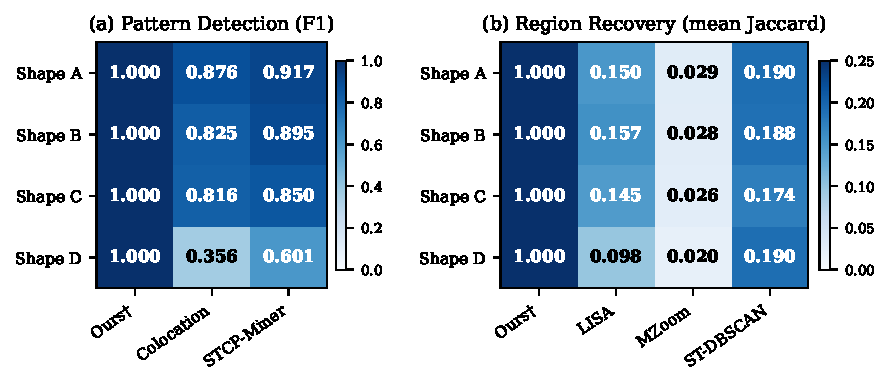
\includegraphics[width=\columnwidth]{fig/fig_ex1_heatmap.pdf}
\caption{EX-1の結果（3シード平均、$p_{\mathrm{embed}}{=}0.25$）。
  (a)~EX-1-1 F1；(b)~EX-1-2 平均Jaccard。
  GTはスライディング窓定義（定義3--5）に基づく厳密解。
  $\dagger$提案手法は定義により厳密解を出力するため F1 $= 1.00$、Jaccard $= 1.00$。
  各比較手法はグリッドサーチで最大スコアのパラメータを採用。}
\label{fig:ex1}
\end{figure}

\paragraph{分析.}
Fig.~\ref{fig:ex1}に各形状・各手法のスコア（3シード平均）を示す。
\emph{EX-1-1（パターン検出F1）。}
Colocationは特にShape D（拡大）で最低となる。
密集の拡大過程でグローバルPI計算が全期間にわたって希釈されるためである。
STCP-Minerは時間ウィンドウで希釈を部分的に回避し改善するが、近似誤差は残る。

\emph{EX-1-2（密集領域復元・平均Jaccard）。}
既存手法は全形状で低スコアにとどまる。

\textbf{LISA}は全時刻の出現を集約して時間情報を失うため，密集範囲を復元できない。

\textbf{MZoom}が最も低スコアとなる。
$S{=}100$のグリッドに対して密集帯が5セル幅であるため、
直積ブロック制約のもとでは帯全体を覆う矩形ブロックを取ると密度が著しく低下する。
その結果、貪欲探索は単一列（幅1）のブロックに収束し、
帯の大部分を偽陰性として見落とす。

\textbf{ST-DBSCAN}は出現セルのみをクラスタメンバとしてラベルするため、
密集ウィンドウ内の非出現セル（密集領域の構成要素の大部分）を系統的に見落とす。

以上の低スコアはパラメータ調整の問題ではなく、
各手法がスライディング窓定義とは本質的に異なる出力を生成するという
構造的なミスマッチに起因する。
同一カテゴリ内の高速化手法も同じ制約を共有するため、
追加しても結果は等価となる（\S\ref{sec:related}）。

% ==============================================================
\subsection{EX-2：スケーラビリティ（合成データ）}
\label{sec:ex2}
% ==============================================================

\paragraph{目的.}
時間格子点数$T$、空間格子点数$S$、次元数$d$、アイテム数$|\mathcal{I}|$の
4パラメータそれぞれについて、
計算時間とピークメモリがどのようにスケールするかを独立に検証する。

\paragraph{合成データ生成.}
$d$次元格子上で、各アイテムを全セルに対して独立に
Bernoulli$(p_{\mathrm{item}}{=}0.10)$からサンプリングし1バスケットを構成する。
空セルにはアイテム1を割り当て、各セルに正確に1トランザクションが存在することを保証する
（生成の詳細はAppendix~\ref{sec:ex2_data_details}）。

\paragraph{提案手法のパラメータ.}
$W = (24, 4)$、$\theta = 15$を全実験で固定。
基準設定：$T{=}1{,}000$、$S{=}100$、$d{=}2$、$|\mathcal{I}|{=}20$。

\paragraph{実験設計.}
4軸を独立に変化させる：
(a)~$T \in \{10^2, 10^3, 10^4, 10^5\}$（$S{=}100$、$d{=}2$固定）；
(b)~$S \in \{10, 10^2, 10^3, 10^4\}$（$T{=}1{,}000$、$d{=}2$固定）；
(c)~$d \in \{2, 3, 4\}$（空間次元を調整して$N{\approx}10^5$を固定）；
(d)~$|\mathcal{I}| \in \{20, 40, 60, 80\}$（$T{=}1{,}000$、$S{=}100$、$d{=}2$固定）。

\paragraph{分析.}
Fig.~\ref{fig:ex2_scalability}に4軸の計算時間とピークRSSを示す。

\emph{(a)(b) T・Sスケーラビリティ.}
実行時間・ピークメモリともに$N$に対しておおむね線形にスケールする。
$N$が$10^4$から$10^7$へ$10^3$倍増加すると、
実行時間は$0.046$\,sから$49.5$\,sへ（${\approx}10^3$倍）、
ピークメモリは$4.9$\,MBから$2{,}135$\,MBへと増加する。
$N{=}10^8$（$T{=}10^6$、$S{=}100$）の拡張実行では$517$\,s（$<9$分）で完了し、
線形スケーリングと整合する。
同一$N$での$T/S$比率の影響として、
$N{=}10^7$において$T{=}10^5$/$S{=}10^2$が$49.5$\,sであるのに対し
$T{=}10^3$/$S{=}10^4$は$59.8$\,s（$1.21$倍）であり、
$T$が大きいほど$t$軸ストライド（Lemma~\ref{lem:stride}）による
ギャップスキップが有効に働く。

\emph{(c) dスケーラビリティ.}
$N{\approx}10^5$を固定した状態で$d$を$2$から$4$へ増やすと、
$W_{\mathrm{sp}}$は$5$から$125$（$25$倍）に増加するが、
ピークメモリは$26$\,MBから$35$\,MB（$1.35$倍）の増加にとどまる。
これは各空間始点のマルチセットが疎であるため、
$W_{\mathrm{sp}}$の増加がメモリに直結しないことを示す。

\emph{(d) $|\mathcal{I}|$スケーラビリティ.}
$|\mathcal{I}|$が$20$から$80$へ増加すると実行時間は$0.44$\,sから$6.8$\,sへ増加する。
指数的増加よりも大幅に緩やかであり、
Aprioriプルーニングが非密集パターンの候補生成を抑制しているためである。

\begin{figure}[t]
\centering
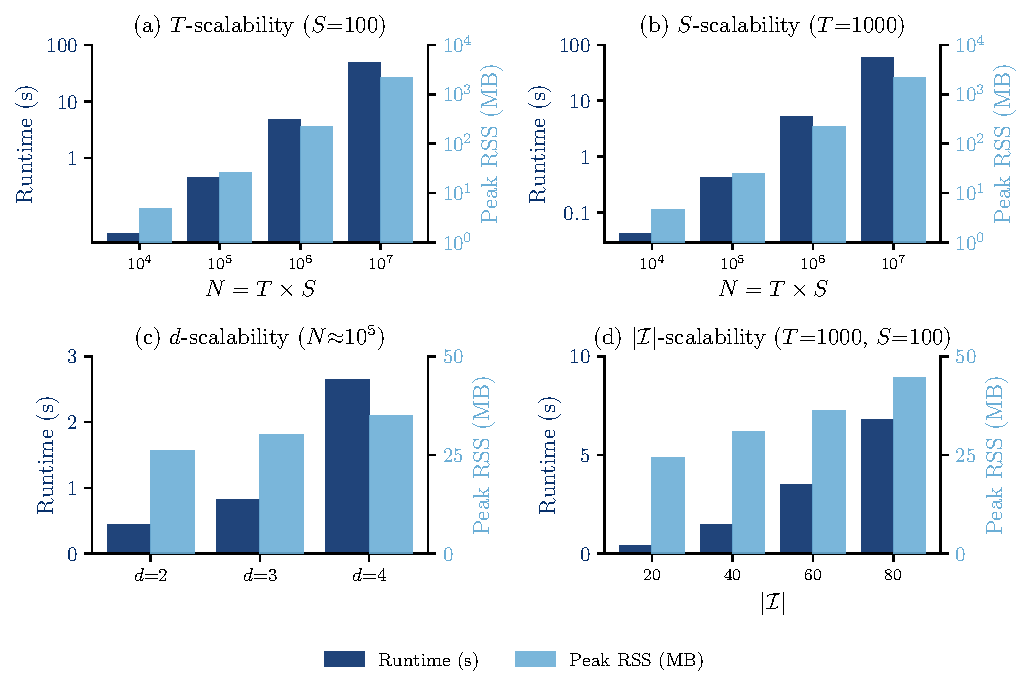
\includegraphics[width=\columnwidth]{fig/fig_ex2_scalability.pdf}
\caption{EX-2：4パラメータのスケーラビリティ
  （$W{=}(24,4)$、$\theta{=}15$、$p_{\mathrm{item}}{=}0.10$）。
  濃青棒：計算時間（左軸）、水色棒：ピークRSS（右軸）。}
\label{fig:ex2_scalability}
\end{figure}

% ==============================================================
\subsection{EX-3：実データへの適用（$d{=}3$--$4$）}
\label{sec:ex3}
% ==============================================================

\paragraph{目的.}
提案手法を多様なドメインの実データに適用し、
検出されたパターンと密集領域がドメイン知識と整合する
解釈可能な示唆を与えることを確認する。

\paragraph{データセットと結果.}
犯罪報告2種（Chicago Crime~\cite{chicagocrime}、NYPD Crime~\cite{nypdcrime}）、
市民苦情（NYC 311~\cite{nyc311}）、
地震カタログ（USGS Earthquake~\cite{usgseq}）の
3ドメイン・$d{=}3$--$4$ の実データセットを使用した。
時間を週単位、空間座標を等幅ビンに離散化し、各セルの発生事象をアイテムとするトランザクションデータに変換した。
データセットの詳細および定量的結果は
付録~\ref{sec:dataset_details}に示す。

\paragraph{得られた示唆.}
Chicago Crimeでは ASSAULT + BATTERY がシカゴ南部・西部に
慢性的な密集ウィンドウを形成し、
3種複合パターン（THEFT + CRIMINAL DAMAGE + BATTERY）により
単独カテゴリ分析では見落とされる複合ホットスポットが特定された。
NYPD Crimeでは重罪と軽犯罪の複合共起が区・週単位で把握され、
NYC 311では騒音苦情と違法駐車の複合パターンが住宅密集地区に繰り返し出現した。
USGS Earthquakeでは深さ軸を含む4次元記述により、
浅発地震と中深発地震を区別した密集パターンが識別された。
いずれの事例でも、提案手法は「どのアイテムセットが、いつ・どこで密集するか」を
具体的な時空間ウィンドウとして出力し、
ドメイン専門家にとって解釈可能な分析結果を与えた。
各データセットの詳細な事例は付録~\ref{sec:real_data_qualitative}に示す。
